\chapter{Methodology}

Construction of associative memory using SNN\cite{base} in this method consist
of four phases
\begin{enumerate}
    \itemsep0em
    \item Initialization: Initialization of SNN and the input spiking signals
    \item Structure formation: New connections with neighbouring neurons are formed
    \item Parameter training: Optimize weight of synapse based on STDP
    \item Pruning: Removing unnecessary connections to improve efficiency
\end{enumerate}
\section{Initialization}
It involves two sub-process in which the data is preprocessed and converted
into spiking signals and the network is initialized.
\subsection{Initialization input spiking signals}
The input to the SNN is spiking signals for that the input values need to be
converted into spiking signals. For the example purpose here MNIST dataset is
used which contains handwritten characters on digits. The figure
\ref{preprocessing} shows the steps involved.

\begin{figure}[h!]
    \centering
    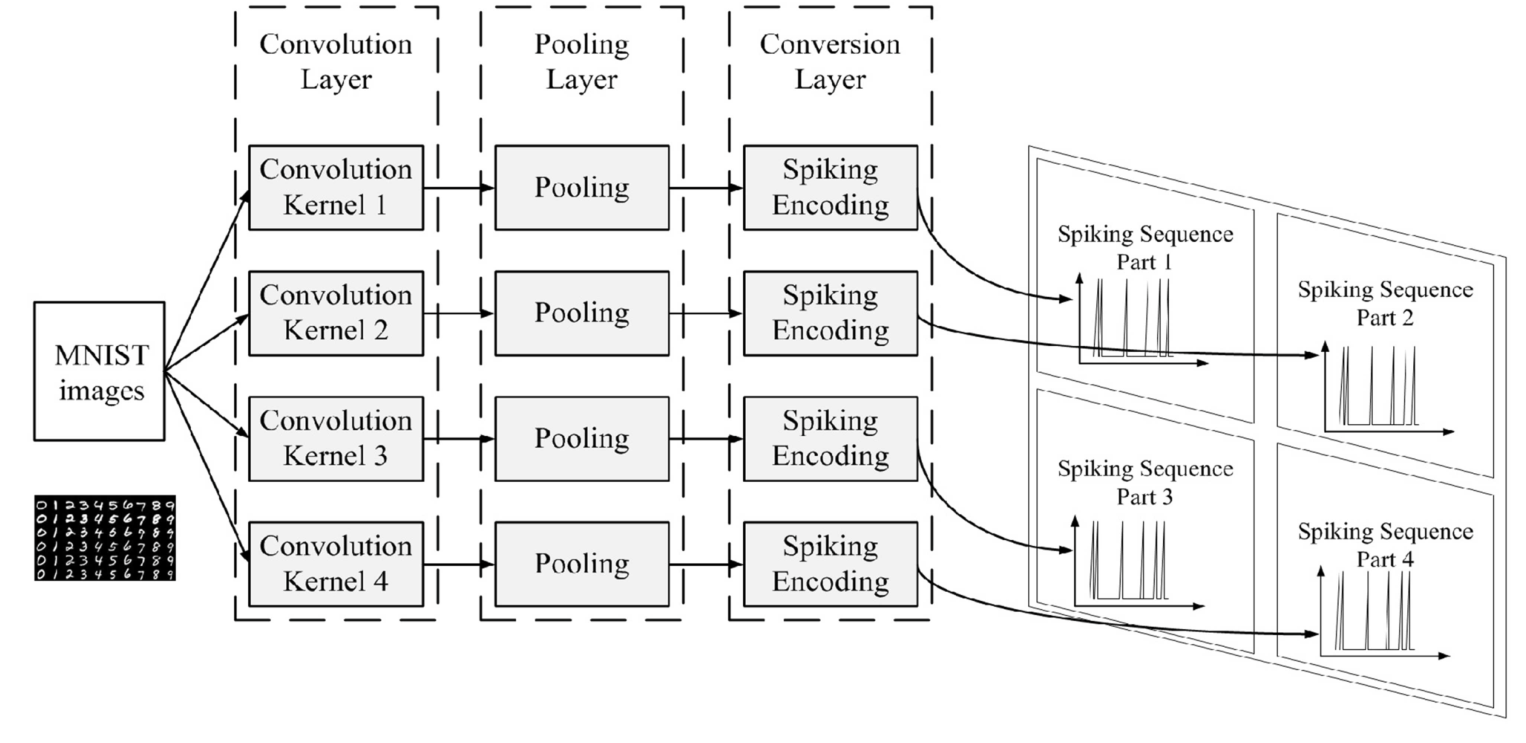
\includegraphics[width=0.8\linewidth]{preprocessing}
    \caption{Data preprocessing}\label{preprocessing}
\end{figure}

Four convolutional kernels of size $4\times4$ shown in figure \ref{kernel} is
applied to the picture pixel values to extract the features. The input image
into the kernel is of size $28\times28$ and the convolutional kernels reduce
the shape into $24\times24$. Next, these values are passed through a maximum
pooling layer shape $2\times2$. It makes the image smaller dimension of
$12\times12$. The conversion layer converts these values into spiking encoding.
Pixel value in the range of [0,255] converted to delay in a spike from
    [0,100]ms. The delay is shorter if value higher.
\begin{figure}[h!]
    \centering
    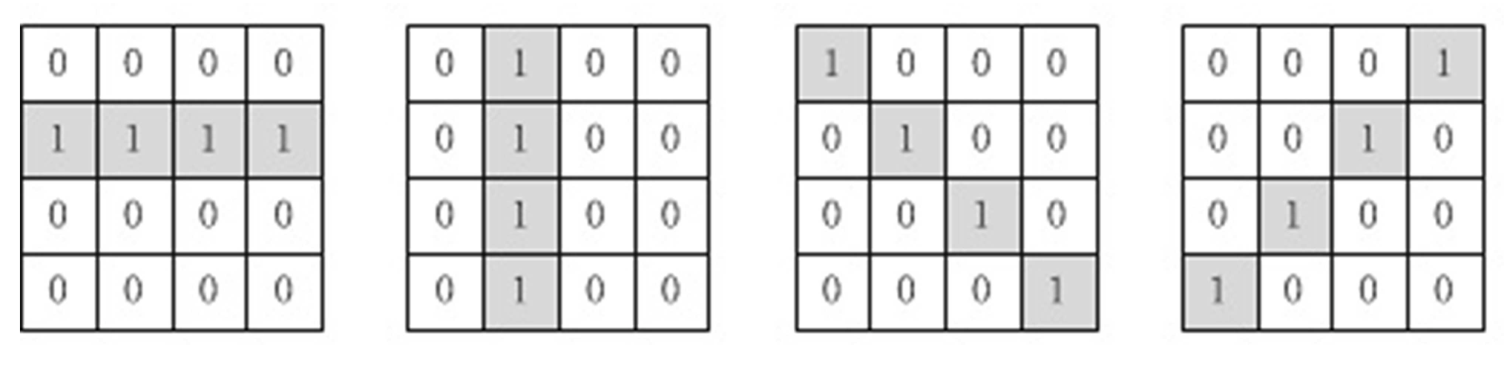
\includegraphics[width=0.8\linewidth]{kernels}
    \caption{Kernels used}\label{kernel}
\end{figure}
To cover the values first min-max normalization is used in which, if
the value of a pixel is d then,
\begin{equation*}
    N(d)=\frac{d-d_{\min}}{d_{\max}-d_{\min}}
\end{equation*}

Where $d_{\min}$ and $d_{\max}$ are maximum and minimum pixel values. Power
encoding is used to get the spike time of pixel d,
\begin{equation*}
    S(d)= (T_{\max}-T_{\min})\times{(N(d)-1)}^2 +T_{\min}
\end{equation*}
where $T_{\min}$ and $T_{\max}$ are the spike's beginning and ending times.
\subsection{Initialization of Spiking neural network}
As shown in figure \ref{structure}, the memory NN in this approach has three
layers: input, memory, and output. The input layer receives the input of the
spiking signal. For the neuron, the LIF model is used. The memory layer grows
new connections to remember them. The process of producing the output is
handled by the output layer. Both the number of input spiking signals and the
number of neurons in the input and memory layers are equal which is 576. Ten
neurons, which is equal to the number of output classes, make up the output
layer.
\begin{figure}[h!]
    \centering
    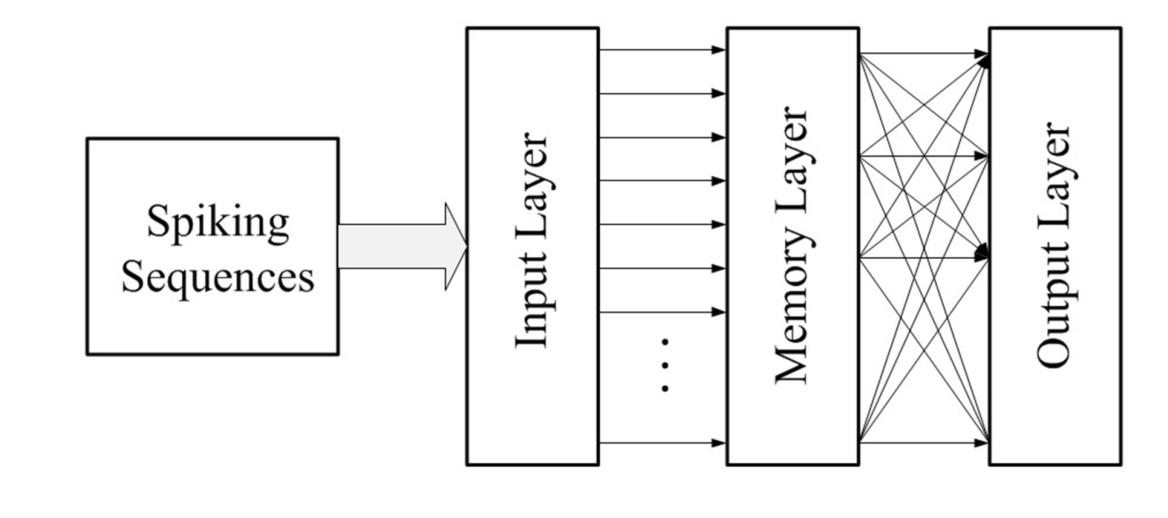
\includegraphics[width=0.8\linewidth]{structure}
    \caption{Structure of network}\label{structure}
\end{figure}

One-to-one connections are made between the input layer and the memory layer.

As a starting point, the synapse's weight is set at 50. It aids in eliciting
the necessary reaction for Hebb's learning rule\cite{hebbs} to take place in
the memory layer.

A coordinate value is given to each neuron in a layer. Using the spatial to
temporal method depicted in the figure\ref{delay}, which encodes the spatial
information of pixel values into the connection delay from the input layer to
the memory layer. The delay in a neuron $i(x,y)$ connection where the pixel
values in an image's x and y coordinates $p \times q$ input layer to the the
corresponding neuron in the memory layer is calculated as
\begin{equation*}
    d_{im(x,y)}=1+p*x+y
\end{equation*}
\begin{figure}[h!]
    \centering
    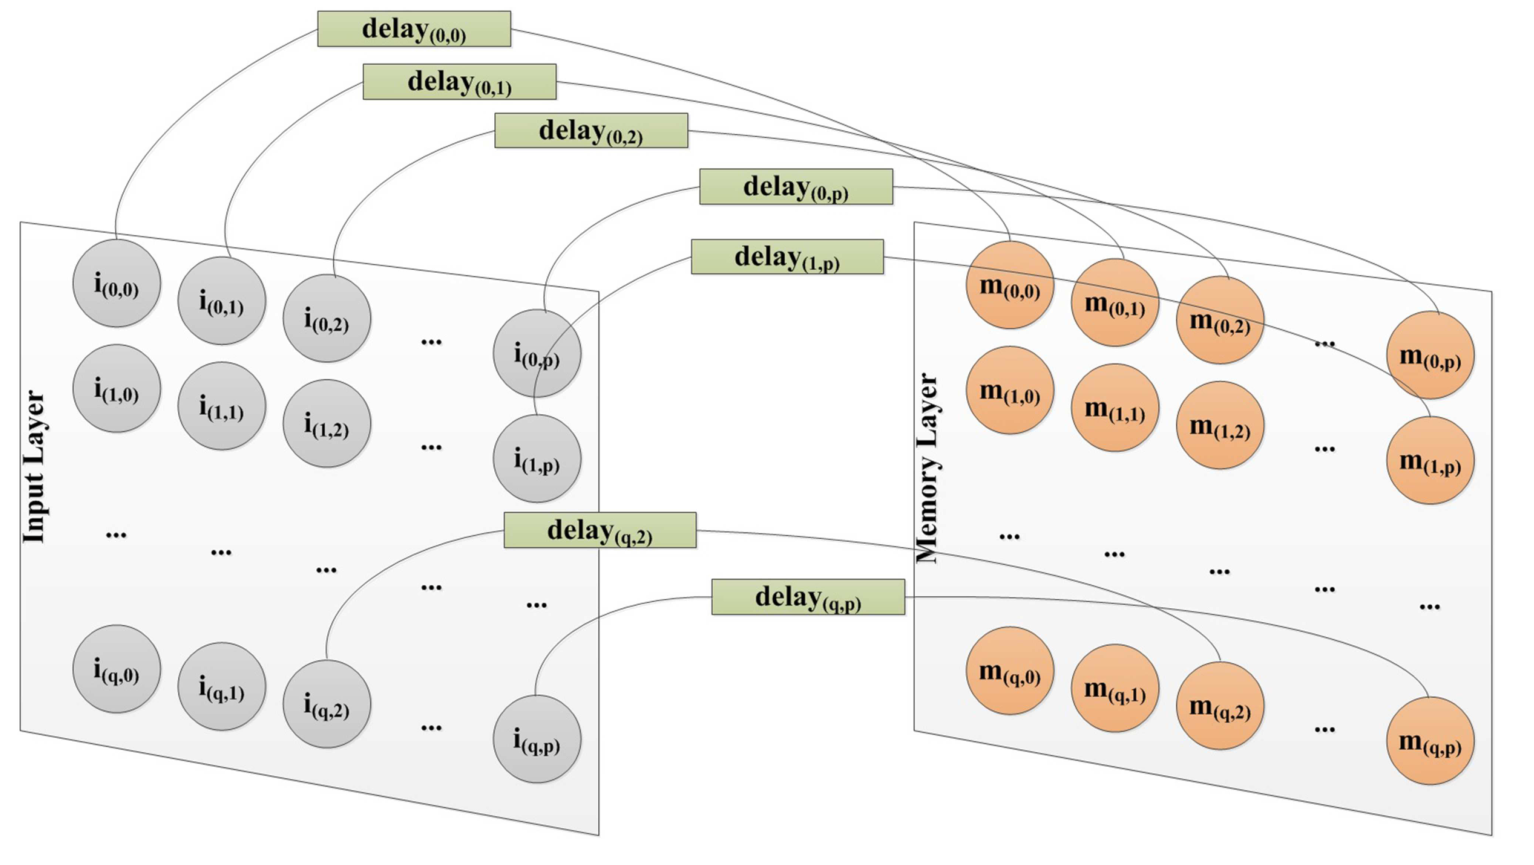
\includegraphics[width=0.8\linewidth]{delay}
    \caption{Delay in neuron connections}\label{delay}
\end{figure}
\section{Forming network structures}
Spiking signals are fed into the network during this phase. The behaviour of
neurons in the memory layer is recorded, and new connections are made within
the memory layer based on Hebb's learning rule\cite{hebbs}. New connection
conditions are based on their threshold values of distance and time difference
in firing two neurons to avoid explosive growth of connections. A new
connection is made between two neurons if they meet the threshold requirements
for firing delay and firing distance but do not already have one.The smaller
the threshold lesser the number of connections that will be created.

Up until the stopping condition is met, it is repeated. Due to the LIF model's
leaky properties, the connection between the memory layer and output layer uses
the previously discussed spatial-to-temporal technique. The calculation of the
connection delay between the memory layer and the output layer is
\begin{equation*}
    d_{mo(x,y)}=1+[N_m-delay_{im(x,y)}]
\end{equation*}
\section{Parameter training}
This phase is based on the ideas of STDP and reinforcement learning. It checks
the recall ability of the network for the set of inputs. This phase does not
change the weights of the connection between layers but rather changes the
weight of the connection within the memory layer itself.The most often fired
neuron in the output layer is taken into consideration as output for this
procedure when a spiking sequence is supplied into the network. If the network
could correctly recall, then there would be no need for optimization;
otherwise, the weights would need to be changed. It works based on the
following algorithm
\begin{description}
    \item[Step 1:] Pick an input image
    \item[Step 2:] Feed input to the network
    \item[Step 3:] Go to step 1 if the output layer's result is accurate; otherwise, go
        to step 4.
    \item[Step 4:] Determine which neurons in the output layer $S_{O}$ and memory layer
        $S_{M}$ are firing inappropriately.
    \item[Step 5:] If i is a neuron in the set $S_M$ and j is a neuron in the set $S_O$
        and the strength of the connection between them is $W_{i,j}$, then
        $W_{i,j}=Shrink\_Coeff*W_{i,j}$
\end{description}This process repeated for all
the images. The value of $Shrink\_Coeff$ is constant between 0 and
1. Figure \ref{recall} demonstrates the memory layer's firing behaviour after receiving an input image corresponding to the number six. Colours indicate
the time at which the spike occurred and lines indicate the connection between
neurons.
\begin{figure}[h!]
    \centering
    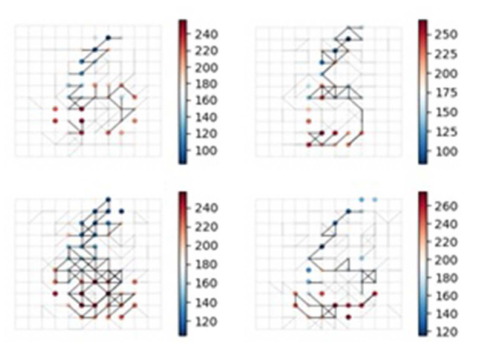
\includegraphics[width=0.8\linewidth]{recall}
    \caption{Recall response for number 6}\label{recall}
\end{figure}
\section{Pruning}
This phase helps in improving the efficiency of the network. If a connection's
weight falls below the threshold during this period (here 3), the connection
will be removed. The connection from the input layer to any memory layer
neurons that don't have any connections to the output layer will likewise be
eliminated.